Vamos utilizar um conjunto de dados sobre supercondutividade, onde carregamos os dados pelo comando abaixo:
\begin{longlisting}
    \begin{minted}{python}
    if 'google.colab' in str(get_ipython()):
        !git clone https://github.com/tiagofiorini/MLinPhysics.git
        import os as os
        os.chdir('./MLinPhysics')
    \end{minted}
\end{longlisting}
\begin{verbatim}
    Cloning into 'MLinPhysics'...
    remote: Enumerating objects: 117, done.
    remote: Counting objects: 100% (43/43), done.
    remote: Compressing objects: 100% (19/19), done.
    remote: Total 117 (delta 31), reused 24 (delta 24), pack-reused 74 (from 1)
    Receiving objects: 100% (117/117), 29.16 MiB | 28.68 MiB/s, done.
    Resolving deltas: 100% (43/43), done.
\end{verbatim}

\begin{longlisting}
    \begin{minted}{python}
    import pandas as pd

    dados = pd.read_csv('Superconductivity.csv')
    \end{minted}
\end{longlisting}

Antes de começar a analisar e tratar os dados, é necessário verificar a existência ou não de valores ausentes no conjunto.
\begin{longlisting}
    \begin{minted}{python}
    print(dados.info())
    \end{minted}
\end{longlisting}
\begin{verbatim}
    <class 'pandas.core.frame.DataFrame'>
    RangeIndex: 21263 entries, 0 to 21262
    Data columns (total 82 columns):
    #   Column                           Non-Null Count  Dtype  
    ---  ------                           --------------  -----  
    0   number_of_elements               21263 non-null  int64  
    1   mean_atomic_mass                 21263 non-null  float64
    2   wtd_mean_atomic_mass             21263 non-null  float64
    3   gmean_atomic_mass                21263 non-null  float64
    4   wtd_gmean_atomic_mass            21263 non-null  float64
    5   entropy_atomic_mass              21263 non-null  float64
    6   wtd_entropy_atomic_mass          21263 non-null  float64
    7   range_atomic_mass                21263 non-null  float64
    8   wtd_range_atomic_mass            21263 non-null  float64
    9   std_atomic_mass                  21263 non-null  float64
    10  wtd_std_atomic_mass              21263 non-null  float64
    11  mean_fie                         21263 non-null  float64
    12  wtd_mean_fie                     21263 non-null  float64
    13  gmean_fie                        21263 non-null  float64
    14  wtd_gmean_fie                    21263 non-null  float64
    15  entropy_fie                      21263 non-null  float64
    16  wtd_entropy_fie                  21263 non-null  float64
    17  range_fie                        21263 non-null  float64
    18  wtd_range_fie                    21263 non-null  float64
    19  std_fie                          21263 non-null  float64
    20  wtd_std_fie                      21263 non-null  float64
    21  mean_atomic_radius               21263 non-null  float64
    22  wtd_mean_atomic_radius           21263 non-null  float64
    23  gmean_atomic_radius              21263 non-null  float64
    24  wtd_gmean_atomic_radius          21263 non-null  float64
    25  entropy_atomic_radius            21263 non-null  float64
    26  wtd_entropy_atomic_radius        21263 non-null  float64
    27  range_atomic_radius              21263 non-null  int64  
    28  wtd_range_atomic_radius          21263 non-null  float64
    29  std_atomic_radius                21263 non-null  float64
    30  wtd_std_atomic_radius            21263 non-null  float64
    31  mean_Density                     21263 non-null  float64
    32  wtd_mean_Density                 21263 non-null  float64
    33  gmean_Density                    21263 non-null  float64
    34  wtd_gmean_Density                21263 non-null  float64
    35  entropy_Density                  21263 non-null  float64
    36  wtd_entropy_Density              21263 non-null  float64
    37  range_Density                    21263 non-null  float64
    38  wtd_range_Density                21263 non-null  float64
    39  std_Density                      21263 non-null  float64
    40  wtd_std_Density                  21263 non-null  float64
    41  mean_ElectronAffinity            21263 non-null  float64
    42  wtd_mean_ElectronAffinity        21263 non-null  float64
    43  gmean_ElectronAffinity           21263 non-null  float64
    44  wtd_gmean_ElectronAffinity       21263 non-null  float64
    45  entropy_ElectronAffinity         21263 non-null  float64
    46  wtd_entropy_ElectronAffinity     21263 non-null  float64
    47  range_ElectronAffinity           21263 non-null  float64
    48  wtd_range_ElectronAffinity       21263 non-null  float64
    49  std_ElectronAffinity             21263 non-null  float64
    50  wtd_std_ElectronAffinity         21263 non-null  float64
    51  mean_FusionHeat                  21263 non-null  float64
    52  wtd_mean_FusionHeat              21263 non-null  float64
    53  gmean_FusionHeat                 21263 non-null  float64
    54  wtd_gmean_FusionHeat             21263 non-null  float64
    55  entropy_FusionHeat               21263 non-null  float64
    56  wtd_entropy_FusionHeat           21263 non-null  float64
    57  range_FusionHeat                 21263 non-null  float64
    58  wtd_range_FusionHeat             21263 non-null  float64
    59  std_FusionHeat                   21263 non-null  float64
    60  wtd_std_FusionHeat               21263 non-null  float64
    61  mean_ThermalConductivity         21263 non-null  float64
    62  wtd_mean_ThermalConductivity     21263 non-null  float64
    63  gmean_ThermalConductivity        21263 non-null  float64
    64  wtd_gmean_ThermalConductivity    21263 non-null  float64
    65  entropy_ThermalConductivity      21263 non-null  float64
    66  wtd_entropy_ThermalConductivity  21263 non-null  float64
    67  range_ThermalConductivity        21263 non-null  float64
    68  wtd_range_ThermalConductivity    21263 non-null  float64
    69  std_ThermalConductivity          21263 non-null  float64
    70  wtd_std_ThermalConductivity      21263 non-null  float64
    71  mean_Valence                     21263 non-null  float64
    72  wtd_mean_Valence                 21263 non-null  float64
    73  gmean_Valence                    21263 non-null  float64
    74  wtd_gmean_Valence                21263 non-null  float64
    75  entropy_Valence                  21263 non-null  float64
    76  wtd_entropy_Valence              21263 non-null  float64
    77  range_Valence                    21263 non-null  int64  
    78  wtd_range_Valence                21263 non-null  float64
    79  std_Valence                      21263 non-null  float64
    80  wtd_std_Valence                  21263 non-null  float64
    81  critical_temp                    21263 non-null  float64
    dtypes: float64(79), int64(3)
    memory usage: 13.3 MB
    None
\end{verbatim}

Não tendo, podemos partir pra análise inicial dos dados. É interessante verificar as caracteríticas principais das variáveis.
\begin{longlisting}
    \begin{minted}{python}
    dados.describe()
    \end{minted}
\end{longlisting}
\begin{table}[H]
    \centering
    \begin{tabular}{cccccc}
        \toprule
        \verb|index| & \verb|number_of_elements| & \verb|mean_atomic_mass| & $\cdots$ & \verb|wtd_std_Valence| & \verb|critical_temp|  \\ 
        \midrule
        count & 21263.000000 & 21263.000000 & $\cdots$ & 21263.000000 & 21263.000000 \\
        mean & 4.115224 & 87.557631 & $\cdots$ & 0.673987 & 34.421219 \\
        std & 1.439295 & 29.676497 & $\cdots$ & 0.455580 & 34.254362 \\
        min & 1.000000 & 6.941000 & $\cdots$ & 0.000000 & 0.000210 \\
        25\% & 3.000000 & 72.458076 & $\cdots$ & 0.306892 & 5.365000 \\
        50\% & 4.000000	 & 84.922750 & $\cdots$ & 0.500000 & 20.000000 \\
        75\% & 5.0000000 & 100.404410 & $\cdots$ & 1.020436 & 63.000000 \\
        max & 9.000000 & 208.980400	 & $\cdots$ & 3.000000 & 185.000000 \\
        \bottomrule
    \end{tabular}
\end{table}

Aqui podemos ver que existe uma disparidade nas escalas das variáveis, onde algumas estão em torno de de um pequeno intervalo (\verb|entropy_fie|, por exemplo, que está entre $[0,2.15]$ aproximadanete) e outras em um grande intervalo, de escala muito maior (\verb|wtd_mean_fie|, por exemplo, que está entre $[375.5, 1348]$ aproximadamente). Isto sugere um reescalonamento nos dados.

Sendo a temperatura crítica (\verb|critical_temp|) nossa variável alvo, podemos verificar sua distribuição utilizando as bibliotecas \verb|matplotlib.pyplot| e \verb|seaborn|.
\begin{longlisting}
    \begin{minted}{python}
    import matplotlib.pyplot as plt
    import seaborn as sns

    plt.figure(figsize=(8, 6))
    sns.histplot(dados['critical_temp'])
    plt.title('Distribuição da Temperatura Crítica')
    plt.xlabel('Temperatura Crítica (K)')
    plt.ylabel('Quantidade de Materiais')
    plt.show()
    \end{minted}
\end{longlisting}
\begin{figure}[H]
    \centering
    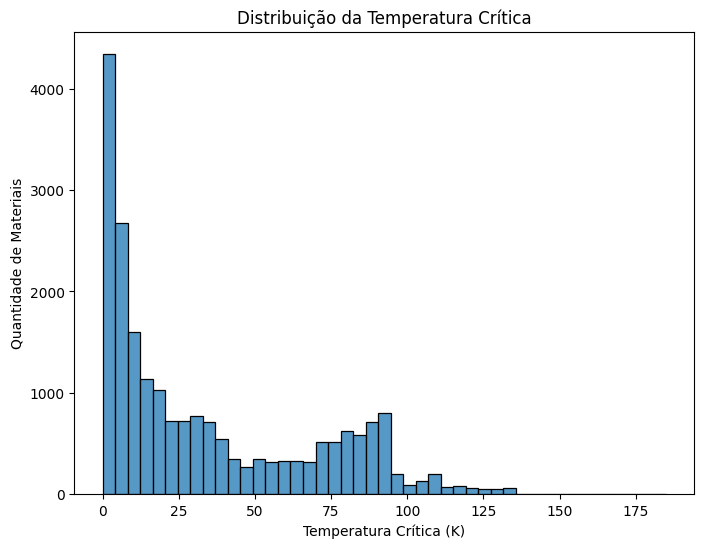
\includegraphics[width=0.8\textwidth]{figures/temperature_distribution.png}
\end{figure}

Vemos nesta distribuição um comportamento relativamente assimétrico, onde há um pico inicial e uma espécie de ``cauda'' conforme a temperatura aumenta, o que sugere uma transformação logaritmica desta variável para normalizar seus valores.

Pela grande quantidade de variáveis do conjunto de dados, seria interessante verificar quais dos atributos possuem maior correlação com a temperatura crítica, o que pode ser feito a partir de um \verb|heatmap|.
\begin{longlisting}
    \begin{minted}{python}
    sns.heatmap(dados.corr(), cmap='inferno')
    plt.title('Correlação entre os atributos')
    plt.show()
    \end{minted}
\end{longlisting}
\begin{figure}[H]
    \centering
    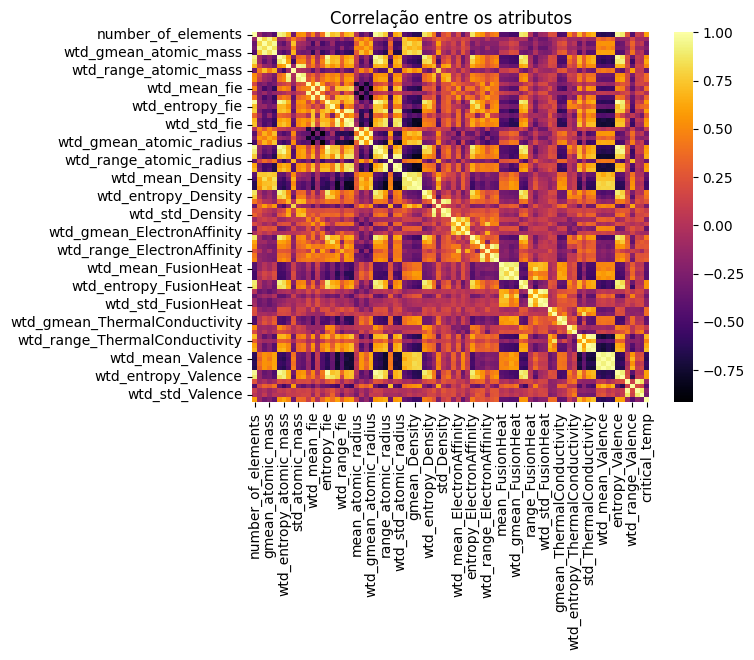
\includegraphics[width=0.8\textwidth]{figures/heatmap.png}
\end{figure}

Pela quantidade de atributos do conjunto de dados, torna-se um pouco difícil estabelecer quais são as variáveis que mais se correlacionam com a temperatura crítica, o que sugere uma outra forma de verificação desta correlação, que pode ser feita com a função \verb|corr()|, verificando quais são os maiores valores (em módulo).
\begin{longlisting}
    \begin{minted}{python}
    import numpy as np

    # Atributos com correlação positiva
    corrTempCrit = dados.corr()['critical_temp'].sort_values(ascending=False)
    print(np.abs(corrTempCrit.head(10+1))) # 10 atributos + temperatura crítica
    \end{minted}
\end{longlisting}
\begin{verbatim}
    critical_temp                  1.000000
    wtd_std_ThermalConductivity    0.721271
    range_ThermalConductivity      0.687654
    range_atomic_radius            0.653759
    std_ThermalConductivity        0.653632
    wtd_entropy_atomic_mass        0.626930
    wtd_entropy_atomic_radius      0.603494
    number_of_elements             0.601069
    range_fie                      0.600790
    wtd_std_atomic_radius          0.599199
    entropy_Valence                0.598591
    Name: critical_temp, dtype: float64
\end{verbatim}
\begin{longlisting}
    \begin{minted}{python}
    # Atributos com correlação negativa
    print(np.abs(corrTempCrit.tail(10).sort_values(ascending=True)))
    \end{minted}
\end{longlisting}
\begin{verbatim}
    wtd_mean_Valence        0.632401
    wtd_gmean_Valence       0.615653
    mean_Valence            0.600085
    gmean_Valence           0.573068
    gmean_Density           0.541684
    wtd_gmean_Density       0.540046
    wtd_range_Valence       0.439901
    wtd_mean_Density        0.433940
    wtd_gmean_FusionHeat    0.432365
    gmean_FusionHeat        0.431795
    Name: critical_temp, dtype: float64
\end{verbatim}

Aqui são mostrados apenas 20 atributos dos 81, sendo eles os primeiros 10 atributos com correlação positiva com a temperatura crítica e os 10 primeiros deles com correlação negativa. O fato de considerarmos atributos com correlações próximas de -1 é que podemos interpretá-los como sendo variáveis que possuem uma correlação inversamente proporcional, por exemplo, pegando a variável \verb|wtd_mean_Valence|, quando ela diminuir, provavelmente a temperatura crítica tende a crescer.

Podemos ver que, em valor absoluto, que um \textit{threshold} de 0.6 na correlação pode indicar uma colinearidade considerável nos atributos do conjunto de dados, o que praticamente se confirma olhando para a diagonal central, onde muitos dos atributos se mostram correlacionados. Levando isto em consideração, temos pelo menos 11 variáveis colinearmente correlacionadas.

Outra pré-análise necessária nestes dados é a verificação de \textit{outliers}, que pode ser verificada com um boxplot retirando a coluna da temperatura crítica.
\begin{longlisting}
    \begin{minted}{python}
    plt.figure(figsize=(20,8))
    sns.boxplot(data=dados.drop(columns=['critical_temp']))
    plt.title('Boxplot das Variáveis')
    plt.xticks(rotation=90)
    plt.show()
    \end{minted}
\end{longlisting}
\begin{figure}[H]
    \centering
    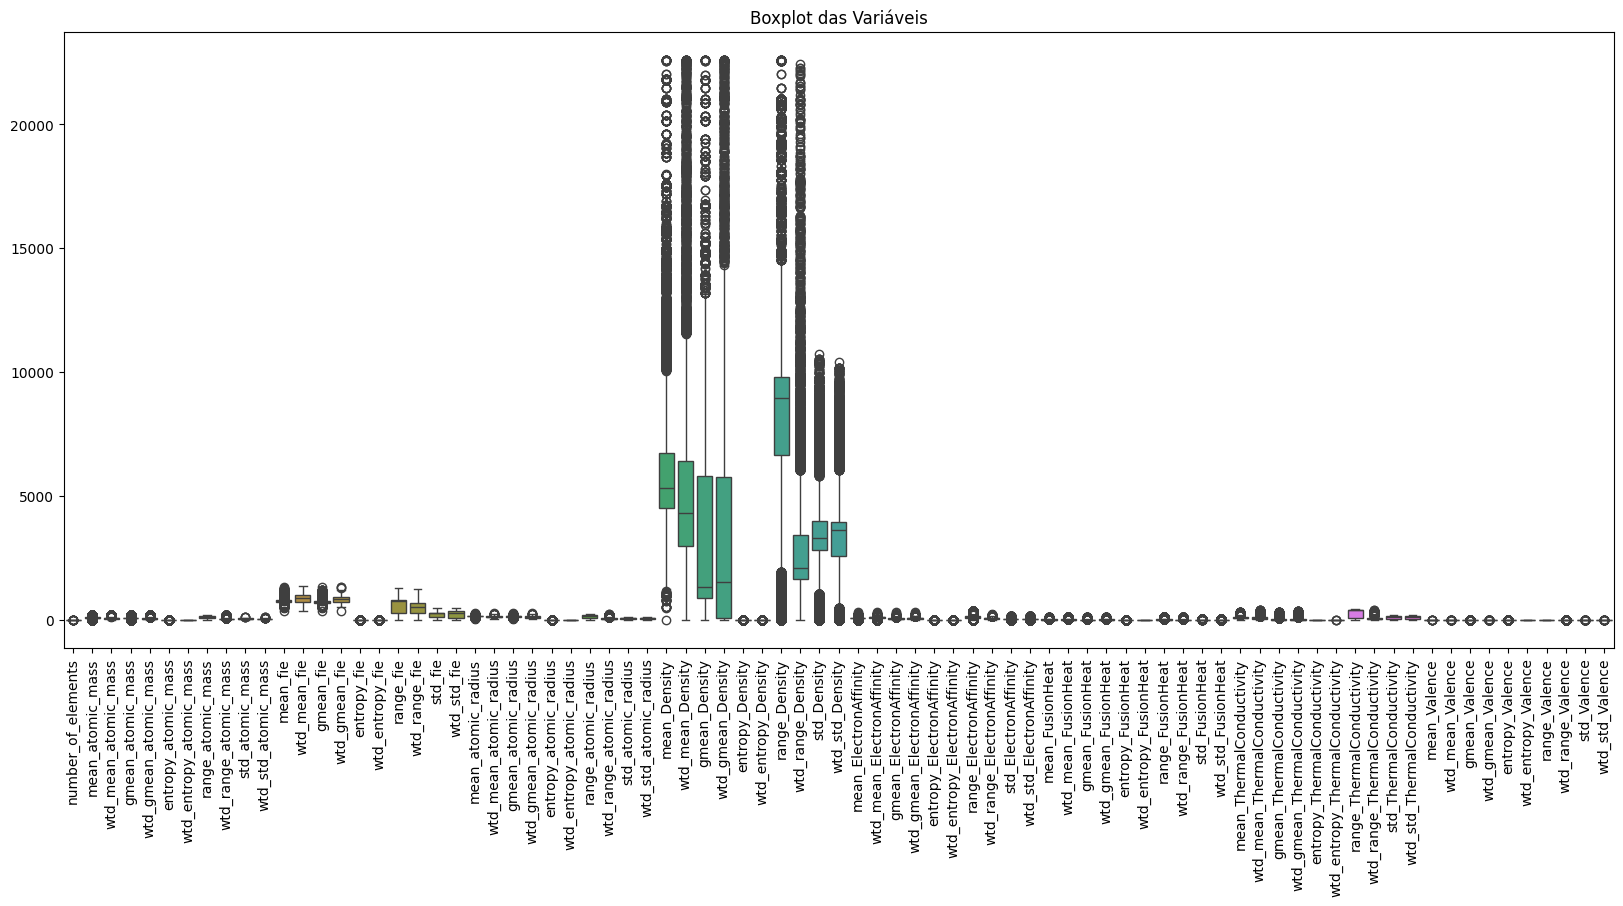
\includegraphics[width=\textwidth]{figures/boxplot.png}
\end{figure}

Mesmo com essa grande quantidade de atributos, ainda conseguimos encontrar uma interpretação para este gráfico. Há sim a presença de \textit{outliers} no conjunto de dados, porém um foco maior estão nas variáveis:
\begin{itemize}
    \item \verb|mean_Density|
    \item \verb|wtd_mean_Density|
    \item \verb|gmean_Density|
    \item \verb|wtd_gmean_Density|
    \item \verb|range_Density|
    \item \verb|wtd_range_Density|
    \item \verb|std_Density|
    \item \verb|wtd_range_Density|
\end{itemize}
o que pode estar associado à alta variabilidade de materiais.